\section{Naive Bayes}
    $\textbf{Naive Bayes}$ è una tecnica semplice per costruire classificatori.
    Non esiste un unico algoritmo per addestrare tali classificatori, ma una famiglia di algoritmi basati su un principio comune: tutti i classificatori $\textit{ingenui}$ (naive) presuppongono che
    il valore di una particolare feature sia $\textbf{indipendente}$ dal valore di qualsiasi altra feature.
    \\[1\baselineskip]
    Prende il nome di Naive Bayes dal $\textbf{Teorema di Bayes}$:
        $$ P \left[ X\ |\ Y \right] = \frac{P \left[ Y\ |\ X \right] \cdot P \left[ X \right]}{P \left[ Y \right]} $$
    
    da cui si può implicare che:
        $$ P \left[ Y\ |\ X \right] \cdot P \left[ X \right] = P \left[ X\ |\ Y \right] \cdot P \left[ Y \right] = P \left[ X,\ Y \right] $$
    \\[1\baselineskip]
    In Machine Learning, il problema si traduce in trovare $P \left[ y\ |\ X \right]$ o, nel caso di molteplici classi $C_{1}, \dots, C_{m}$, trovare
        $$ \arg \max_{C_i} \left[ P \left( C_{i}\ |\ X \right) \right] $$

    Assumendo che ogni feature è condizionalmente indipendente dalle altre:
        $$ P(C_i |X) = P(x_1 | C_i) \cdot P(x_2 | C_i) \cdot \ldots P(x_f | C_i) $$
    
    la predizione del modello sarà:
        $$ \arg \max_{C_i} \left[ P \left( C_{i}\ |\ X \right) \right] = P(x_1 | C_i) \cdot P(x_2 | C_i) \cdot \ldots P(x_f | C_i) \cdot \frac{P(C_i)}{P(X)} $$

    Siccome $P \left( X \right)$ non cambia il ranking delle classi $C_{i}$ possiamo anche rimuoverlo dall'equazione, se per scopi di classificazione:
        $$ \arg \max_{C_i} \left[ P \left( C_{i}\ |\ X \right) \right] = P(x_1 | C_i) \cdot P(x_2 | C_i) \cdot \ldots P(x_f | C_i) \cdot P(C_i) $$

    \clearpage

    \begin{figure}[h]
        \caption[short]{Esempio di classificazione}
        \centering
        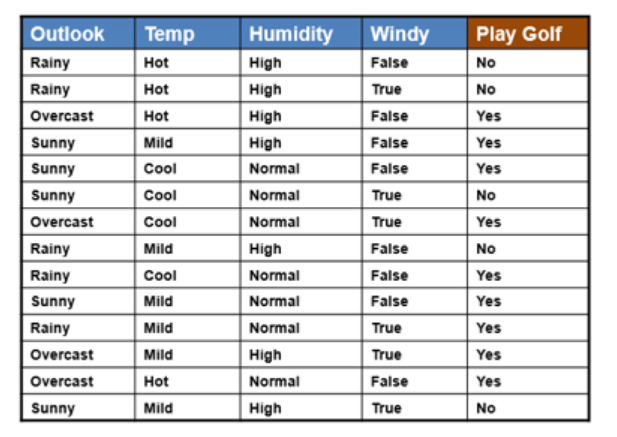
\includegraphics[width = 10cm]{table-bayes-example1.png}
        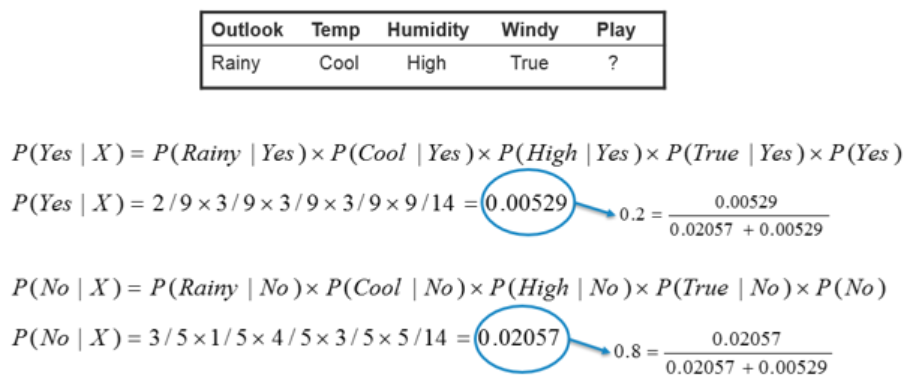
\includegraphics[width = 10cm]{table-bayes-example2.png}
    \end{figure}

    \clearpage

    \subsection{Zero-Frequency Problem}
        Nel caso una certa probabilità $P \left( x_{j}\ |\ C_{i} \right) = 0$, l'intero prodotto andrebbe anch'esso a zero, pure se i segnali delle altre features sono molto forti!
        \\
        Per ovviare a questo problema si utilizza la $\textbf{Correzione di Laplace}$
            $$ P(x_{j}\ |\ C_{i}) = \frac{N_{ij} + 1}{N_{i} + v} $$

        dove:
            \begin{itemize}
                \item $N_{ij}$ è il numero di istanze in classe $C_{i}$ con la $j$-esima feature uguale a $x_{j}$;
                \item $N_{i}$ è il numero di istanze in classe $C_{i}$;
                \item $v$ è il numero totale di valori unici della $j$-esima feature nel dataset $\cal D$.
            \end{itemize}

        $\textbf{Nota:}$ questa correzione deve essere applicata a ogni feature ordinale e non solo a quella per cui accade il problema della frequenza a zero!

    \clearpage